\documentclass[11pt,a4paper]{article}
\usepackage[T2A,T1]{fontenc}
\usepackage[utf8]{inputenc}
\usepackage[english,russian]{babel}
\usepackage{geometry}
\usepackage{graphicx}
\usepackage{booktabs}
\usepackage{microtype}
\usepackage[hidelinks]{hyperref}
\geometry{margin=18mm}
\graphicspath{{results_batch_tau1/}}
\setlength{\parindent}{1.1em}
\setlength{\parskip}{0.25em}
\newcommand{\code}[1]{{\fontencoding{T1}\selectfont\ttfamily #1}}

\title{Сравнительный EDM-анализ режимов обучения nanoGPT\\
Фиксированная задержка $\tau=1$}
\author{Технический отчёт по восьми логам из \code{nanogpt\_muon\_edm}}
\date{30 июля 2026 г.}

\begin{document}
\maketitle

\begin{abstract}
Восемь завершённых nanoGPT-запусков проанализированы единым скользящим
EDM-конвейером при $\tau=1$. Для каждого ряда training loss использованы FNN,
метод Cao, simplex projection и Levina--Bickel MLE, отдельно для исходного и
локально detrended ряда. Логи образуют два размеченных режима: \code{lmo}
при learning rate 0.06 (пять запусков) и \code{sign} при learning rate 0.03
(три запуска). Ни один режим не демонстрирует согласованного позднего
dimensionality collapse: FNN слабо снижается, но simplex и MLE растут во всех
восьми запусках. Это descriptive negative/control result; одиночные запуски
и разные learning rate не позволяют ранжировать оптимизаторы статистически.
\end{abstract}

\section{Данные и методика}

Каждый лог содержит 2330 последовательных наблюдений training loss
(шаги 0--2329) и 11 validation-loss точек. Восстановленный training loss
нормализован к token-level cross-entropy. Для каждого запуска рассчитано
49 скользящих окон: длина 400 шагов, сдвиг 40 шагов. В итоге получено
392 строки оконного анализа.

Во всех окнах использованы фиксированная задержка $\tau=1$, максимальная
размерность embedding $E_{max}=15$ и $k=5$ соседей для MLE. ``Early'' и
``late'' --- средние соответственно первых и последних 12 окон. Анализ
повторён для raw loss и после удаления локального линейного тренда.
Последнее окно имеет центр на шаге 2120, поэтому extension, начинающийся на
шаге 2290, отдельно этим оконным анализом не измеряется.

\begin{figure}[ht]
\centering
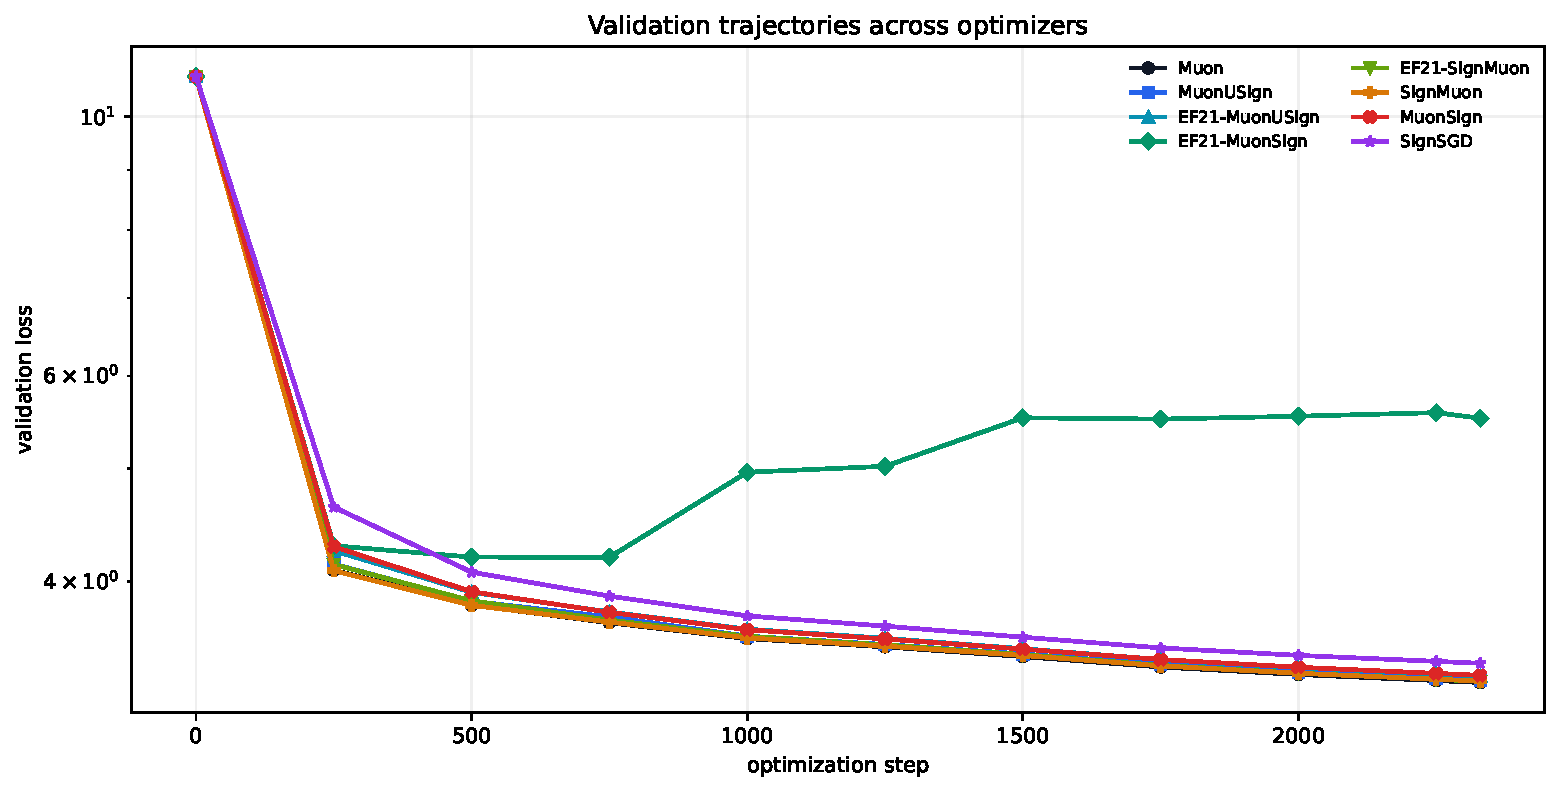
\includegraphics[width=\textwidth]{01_validation_comparison.pdf}
\caption{Validation loss всех восьми запусков.}
\end{figure}

\section{Результаты запусков}

\begin{table}[ht]
\centering
\small
\caption{Итоговые показатели запусков.}
\begin{tabular}{llrrrr}
\toprule
Оптимизатор & Режим & LR & Final val & Best val & Время, s \\
\midrule
Muon              & lmo  & 0.06 & 3.2785 & 3.2785 & 143.8 \\
MuonUSign         & lmo  & 0.06 & 3.2959 & 3.2959 & 143.6 \\
EF21-MuonUSign    & lmo  & 0.06 & 3.3203 & 3.3203 & 144.5 \\
EF21-MuonSign     & lmo  & 0.06 & 5.5198 & 4.1967 & 144.6 \\
EF21-SignMuon     & lmo  & 0.06 & 3.2860 & 3.2860 & 144.5 \\
SignMuon          & sign & 0.03 & 3.2881 & 3.2881 & 144.3 \\
MuonSign          & sign & 0.03 & 3.3249 & 3.3249 & 143.1 \\
SignSGD           & sign & 0.03 & 3.4049 & 3.4049 & 143.2 \\
\bottomrule
\end{tabular}
\end{table}

Семь exact/server-моделей заканчивают в узком диапазоне 3.2785--3.4049.
\code{EF21-MuonSign} требует отдельной интерпретации: exact/server модель
заканчивается на 5.5198, в то время как logged compressed/broadcast модель
$W$ заканчивается на 3.3213. Поэтому среднее final validation loss режима
\code{lmo} искажено этой разницей состояний; его медиана равна 3.2959.

\begin{figure}[ht]
\centering
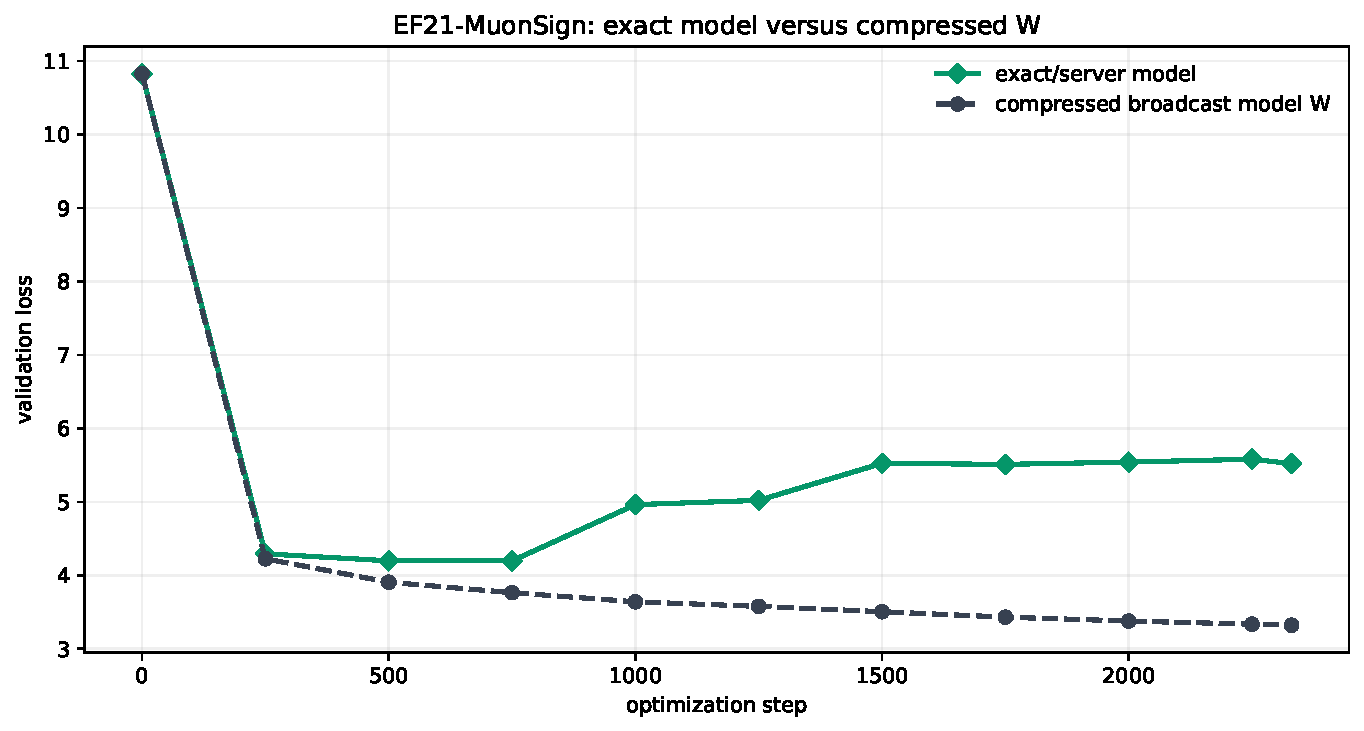
\includegraphics[width=0.82\textwidth]{01b_ef21_muonsign_exact_vs_w.pdf}
\caption{\code{EF21-MuonSign}: exact/server модель и broadcast-модель $W$.}
\end{figure}

\clearpage
\section{Сводка четырёх EDM-методов}

В таблице приведено направление изменения late минус early по всем восьми
оптимизаторам. Абсолютные величины разных методов не являются взаимозаменяемыми:
важна согласованность направления изменения.

\begin{table}[ht]
\centering
\caption{Изменение оценок размерности: late минус early.}
\begin{tabular}{llrrrr}
\toprule
Ряд & Метод & Снижение & Без изм. & Рост & Среднее $\Delta$ \\
\midrule
Raw & FNN     & 5 & 2 & 1 & -0.32 \\
Raw & Cao     & 1 & 0 & 7 & +0.46 \\
Raw & Simplex & 0 & 0 & 8 & +3.61 \\
Raw & MLE     & 0 & 0 & 8 & +1.83 \\
\midrule
Detrended & FNN     & 5 & 1 & 2 & -0.27 \\
Detrended & Cao     & 3 & 0 & 5 & +0.10 \\
Detrended & Simplex & 0 & 0 & 8 & +1.99 \\
Detrended & MLE     & 0 & 0 & 8 & +0.68 \\
\bottomrule
\end{tabular}
\end{table}

Simplex и MLE увеличиваются в каждом запуске как для raw, так и для
detrended loss. FNN является пороговой целочисленной эвристикой, а Cao
выбирает первое плато своей кривой, поэтому их слабые и неоднородные сдвиги
не образуют подтверждения коллапса.

\begin{figure}[ht]
\centering
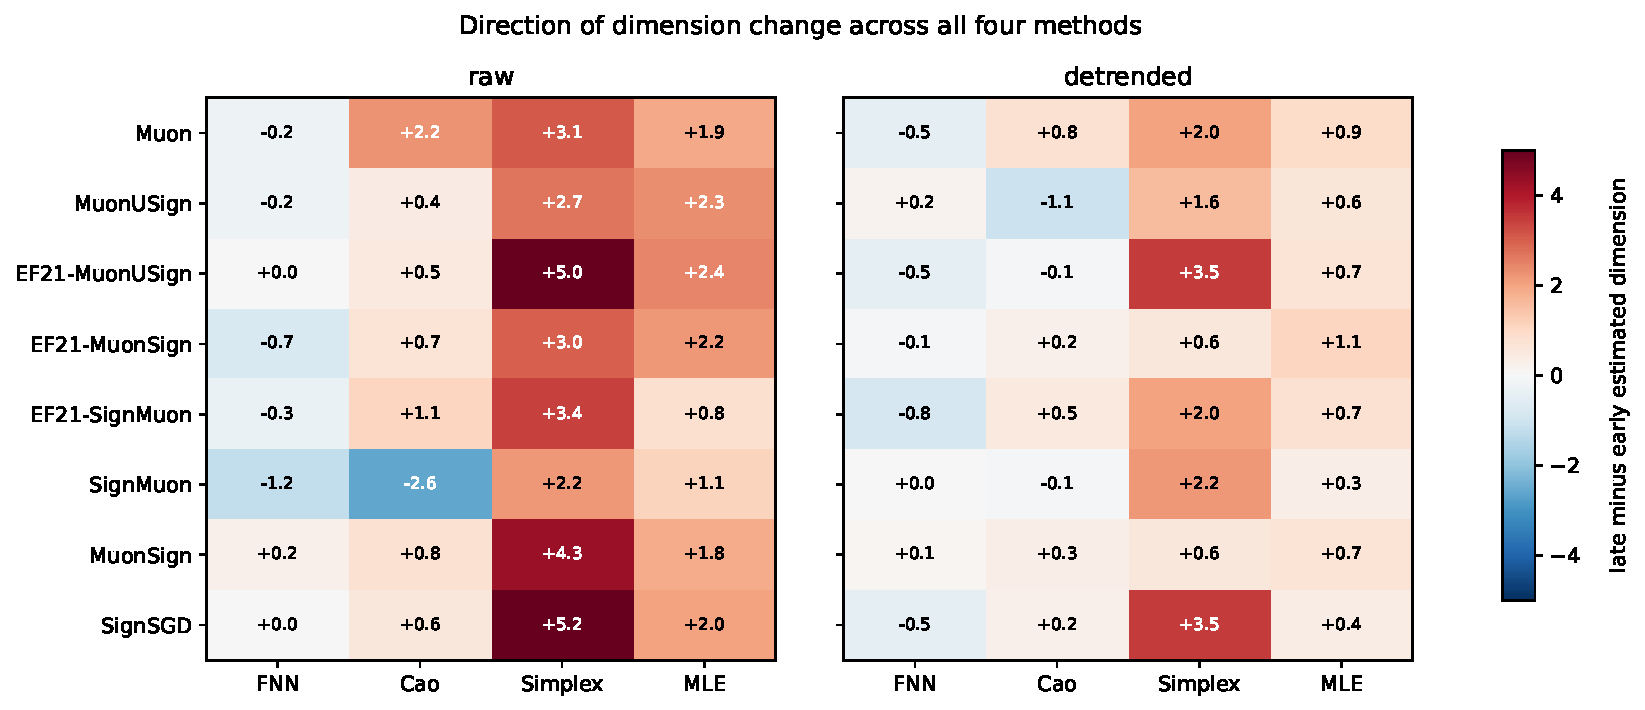
\includegraphics[width=0.90\textwidth]{05_all_method_deltas.pdf}
\caption{Направления изменений по всем четырём методам.}
\end{figure}

\section{MLE по каждому методу оптимизации}

\begin{table}[ht]
\centering
\scriptsize
\caption{Полная сводка MLE. $\Delta$ равно late минус early.}
\begin{tabular}{llrrrrrr}
\toprule
Оптимизатор & Режим & Raw early & Raw late & $\Delta$ & Detr. early & Detr. late & $\Delta$ \\
\midrule
Muon           & lmo  & 12.88 & 14.77 & +1.89 & 14.39 & 15.30 & +0.91 \\
MuonUSign      & lmo  & 13.06 & 15.40 & +2.34 & 14.39 & 15.02 & +0.62 \\
EF21-MuonUSign & lmo  & 12.48 & 14.91 & +2.43 & 14.52 & 15.21 & +0.69 \\
EF21-MuonSign  & lmo  & 12.62 & 14.78 & +2.17 & 14.27 & 15.33 & +1.06 \\
EF21-SignMuon  & lmo  & 13.83 & 14.64 & +0.81 & 14.34 & 15.09 & +0.75 \\
SignMuon       & sign & 13.82 & 14.94 & +1.12 & 14.82 & 15.16 & +0.34 \\
MuonSign       & sign & 12.97 & 14.81 & +1.84 & 14.58 & 15.27 & +0.69 \\
SignSGD        & sign & 12.93 & 14.93 & +2.01 & 14.70 & 15.09 & +0.39 \\
\bottomrule
\end{tabular}
\end{table}

Во всех восьми случаях MLE возрастает. Detrending уменьшает средний рост,
но не меняет его знак; следовательно, даже остаточная локальная геометрия
этого скалярного наблюдаемого не демонстрирует позднего collapse.

\begin{figure}[ht]
\centering
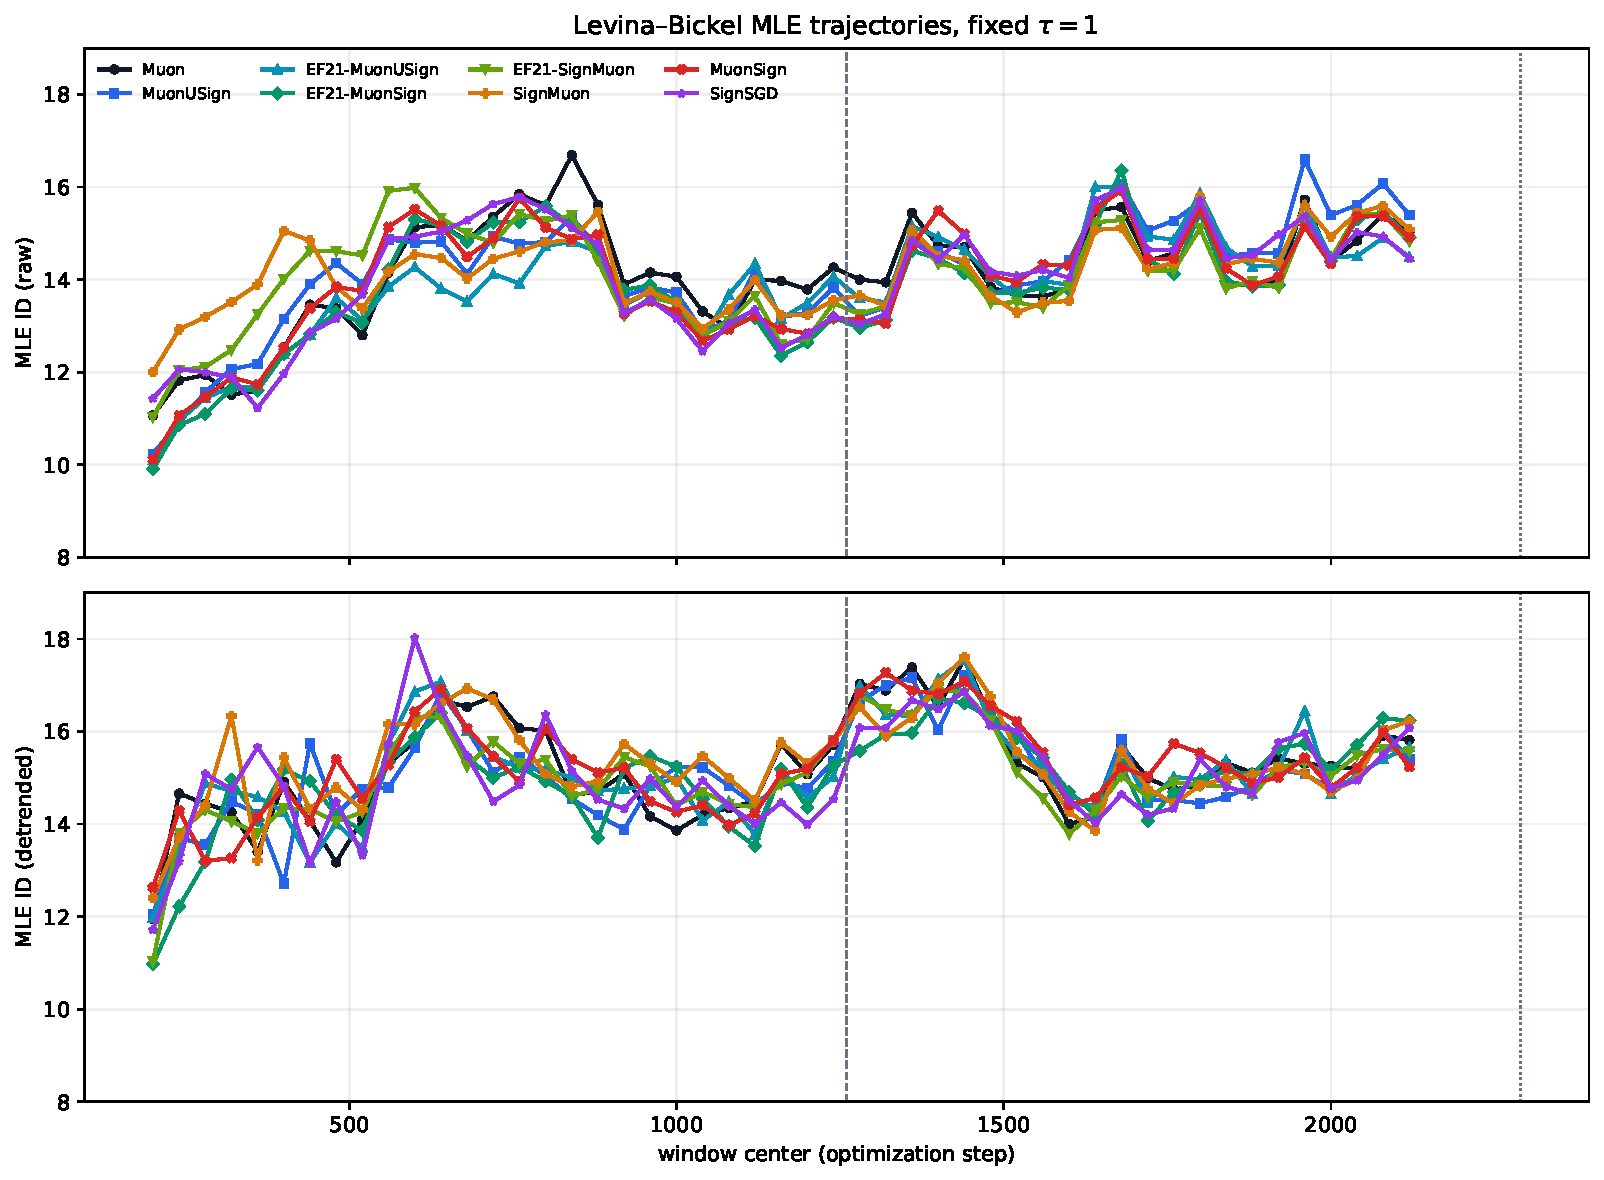
\includegraphics[width=0.88\textwidth]{02_mle_trajectories.pdf}
\caption{Траектории Levina--Bickel MLE для raw и detrended loss.}
\end{figure}

\begin{figure}[ht]
\centering
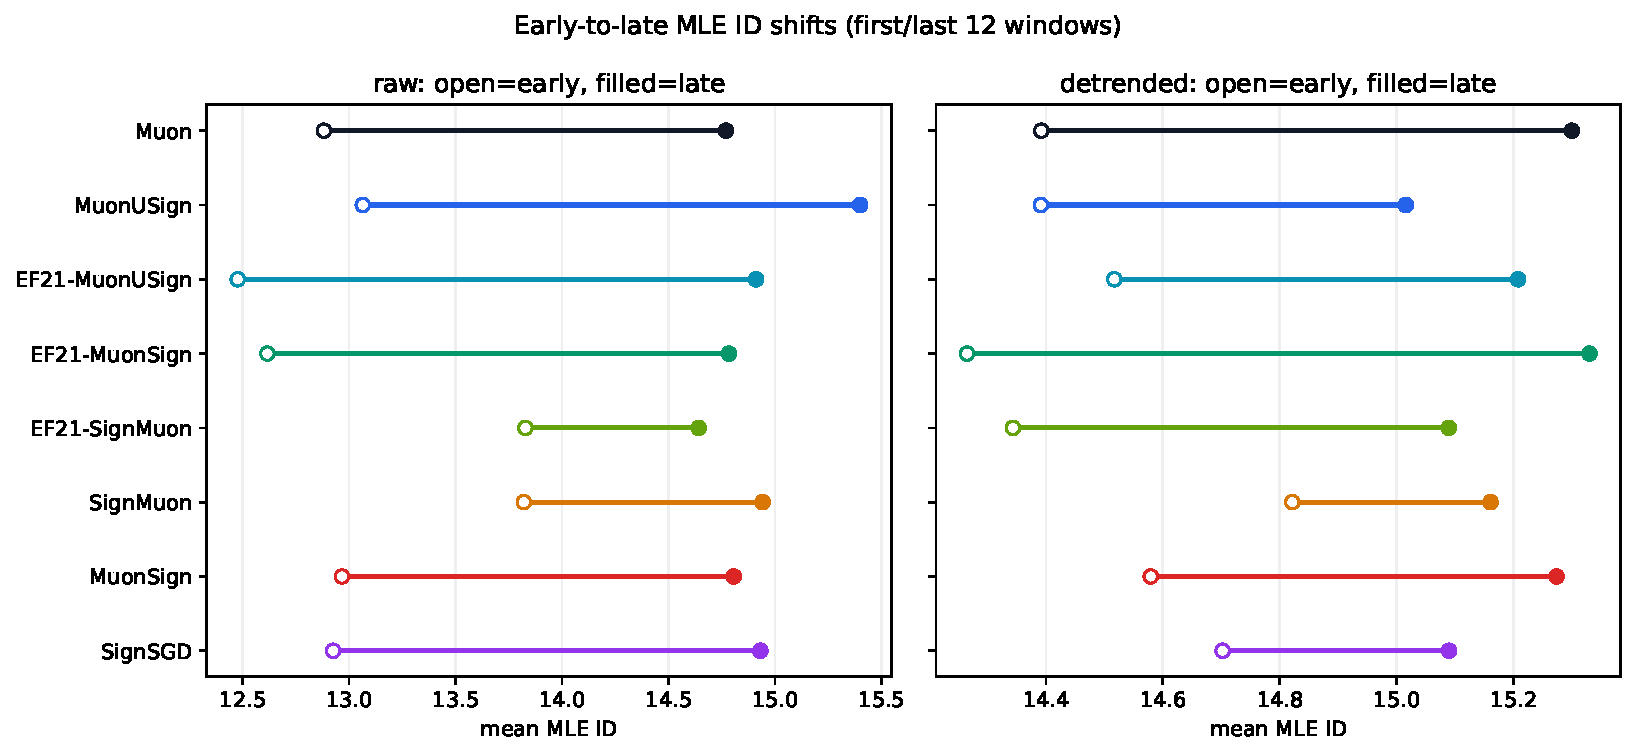
\includegraphics[width=\textwidth]{04_mle_early_late.pdf}
\caption{Ранние и поздние MLE-оценки каждого оптимизатора.}
\end{figure}

\clearpage
\section{Сравнение режимов обучения}

\begin{table}[ht]
\centering
\small
\caption{Описательное сравнение режимов.}
\begin{tabular}{lrrrrrrr}
\toprule
Режим & LR & $n$ & Final mean & Final median & Raw MLE $\Delta$ & Detr. MLE $\Delta$ \\
\midrule
lmo  & 0.06 & 5 & 3.7401 & 3.2959 & +1.93 & +0.81 \\
sign & 0.03 & 3 & 3.3393 & 3.3249 & +1.66 & +0.47 \\
\bottomrule
\end{tabular}
\end{table}

После detrending поздние средние MLE почти совпадают: 15.19 для \code{lmo}
и 15.17 для \code{sign}. Рост несколько больше в \code{lmo} (+0.81 против
+0.47), но это не статистически установленное различие: сравниваются 5 и 3
неоднородных одиночных запуска, а семейство оптимизатора смешано с learning
rate.

\begin{figure}[ht]
\centering
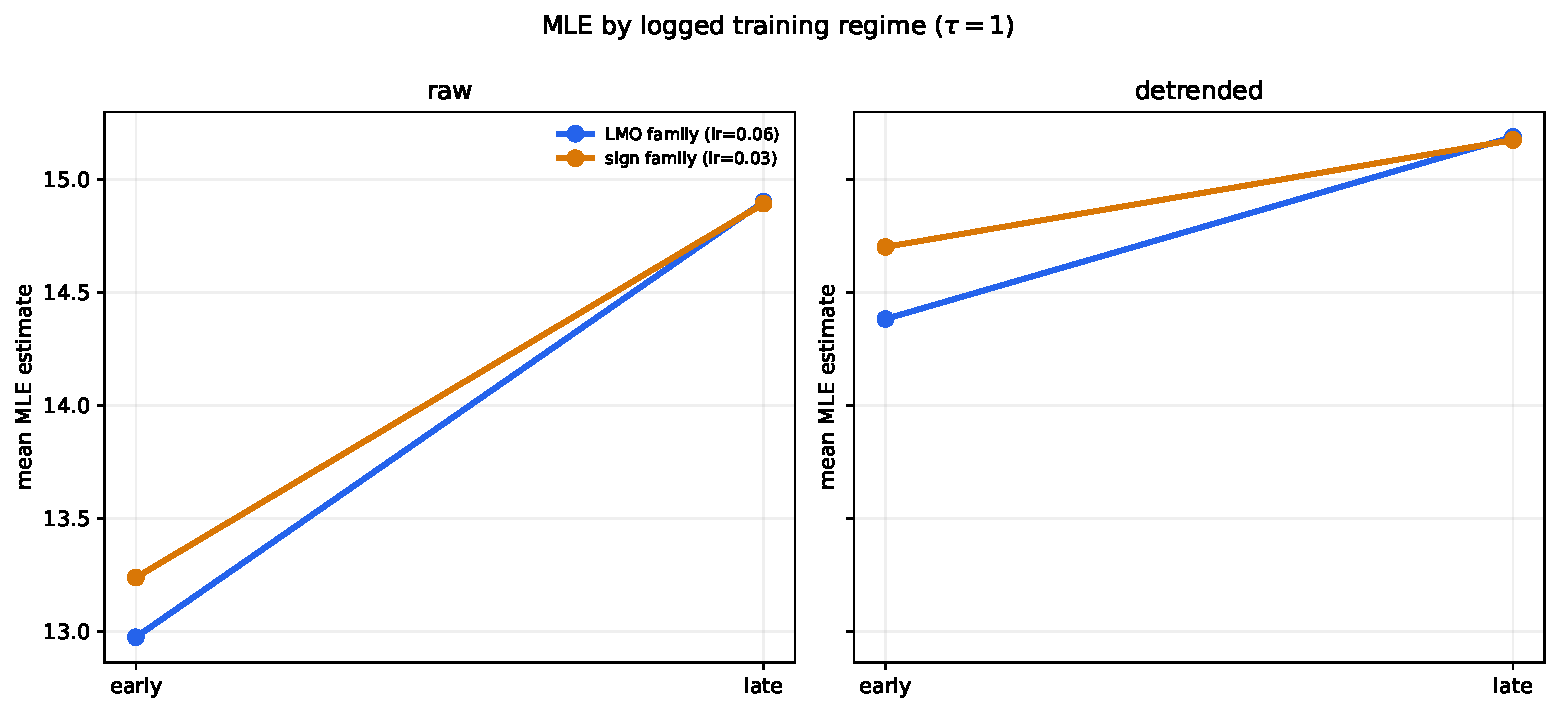
\includegraphics[width=0.88\textwidth]{06_mle_regime_comparison.pdf}
\caption{Средние MLE-оценки двух размеченных режимов.}
\end{figure}

Для остальных методов оба режима сходятся в основной картине: FNN слабо
уменьшается, simplex увеличивается, MLE увеличивается. Cao raw меняет знак
между режимами (+0.98 у \code{lmo}, -0.42 у \code{sign}), однако после
detrending оба сдвига малы (+0.07 и +0.17); это похоже на чувствительность
plateau-правила Cao, а не на надёжное различие динамики обучения.

\section{Ограничения и вывод}

\begin{enumerate}
\item На оптимизатор имеется один запуск; seed не записан.
\item Режимы смешаны с learning rate: \code{lmo}=0.06, \code{sign}=0.03.
\item Окна перекрываются на 90\% и не являются независимыми репликами.
\item Legacy nearest-neighbour методы не используют Theiler window.
\item Simplex часто выбирает границу $E=15$; MLE иногда превышает 15 и
      должен трактоваться как выход эвристики, а не буквальная ID.
\item Скалярный stochastic mini-batch loss не описывает полное состояние
      оптимизатора или геометрию весов.
\end{enumerate}

Таким образом, при фиксированном $\tau=1$ эти восемь nanoGPT-запусков не
демонстрируют estimator-robust позднего dimensionality collapse в скалярном
training loss. Материал годится как negative/control case для статьи:
EDM-вывод зависит от выбранного observable и оценивателя, а не даёт здесь
надёжного способа отличить два режима обучения.

\paragraph{Воспроизводимость.}
Исходные итоговые таблицы: \code{results\_batch\_tau1/optimizer\_run\_summary.csv},
\code{tau1\_early\_late\_all\_methods.csv},
\code{training\_regime\_summary.csv}; полный конвейер ---
\code{analyze\_batch\_tau1.py}.

\end{document}
